\documentclass[11pt]{beamer}
\usepackage[spanish]{babel}

\usepackage{multicol}
\usepackage{tikz}

\mode<presentation> {
  \usetheme{Madrid}
}

\usepackage[spanish]{babel}
\usepackage[utf8]{inputenc}
\usepackage{graphicx} 
\usepackage{booktabs} 



\institute[CIMAT] 
{
%================= logos no meio =====================
%\vspace*{-0.35cm}

\includegraphics[scale=0.12]{img/cimat.png}

\includegraphics[width=1.8cm]{img/seminario_uam.png}
%\hspace*{0.25cm}~%
%\includegraphics[width=1.8cm]{img/logo-neo.png}
\vspace*{0.35cm}\\
Seminario del posgrado en matemáticas UAM-I \\
%\medskip
%\texttt{\{lods.eng,ronety\}@uea.edu.br} % emails
}
\date{\today}

\AtBeginSection[]
{
\begin{frame}
\frametitle{Contenido}
\tableofcontents[currentsection]
\end{frame}
}



\title[Modelos y Arquitecturas]
{Presentación de Modelos y Arquitecturas empleadas para la detección de derrames}

\author[Suárez, Arturo]{Manuel Arturo Suárez Améndola}

\begin{document}

\section{UNet}
\begin{figure}
  \begin{center}
    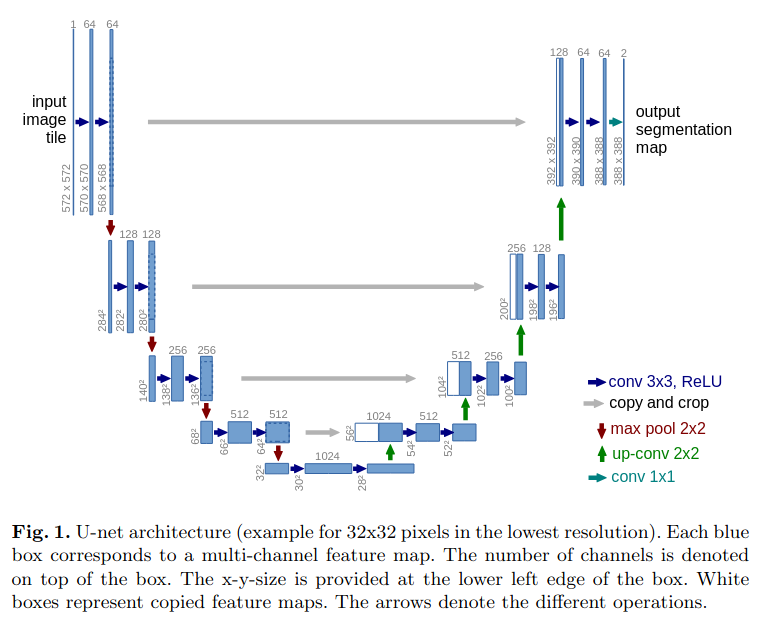
\includegraphics[scale=1.5]{images/unet.png}
  \end{center}
  \caption{UNet}\label{fig:}
\end{figure}

\section{UNet++}
\begin{figure}
  \begin{center}
    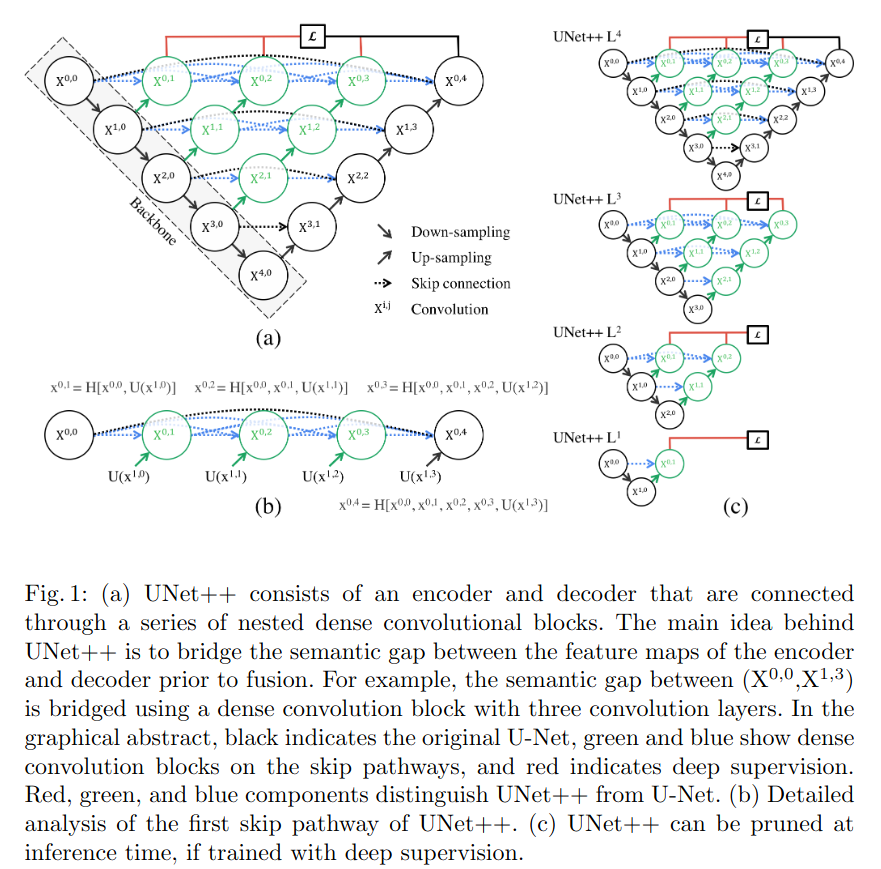
\includegraphics[scale=1.1]{images/unetpp.png}
  \end{center}
  \caption{UNet++}\label{fig:}
\end{figure}

\section{UNet3p}
\begin{figure}
  \begin{center}
    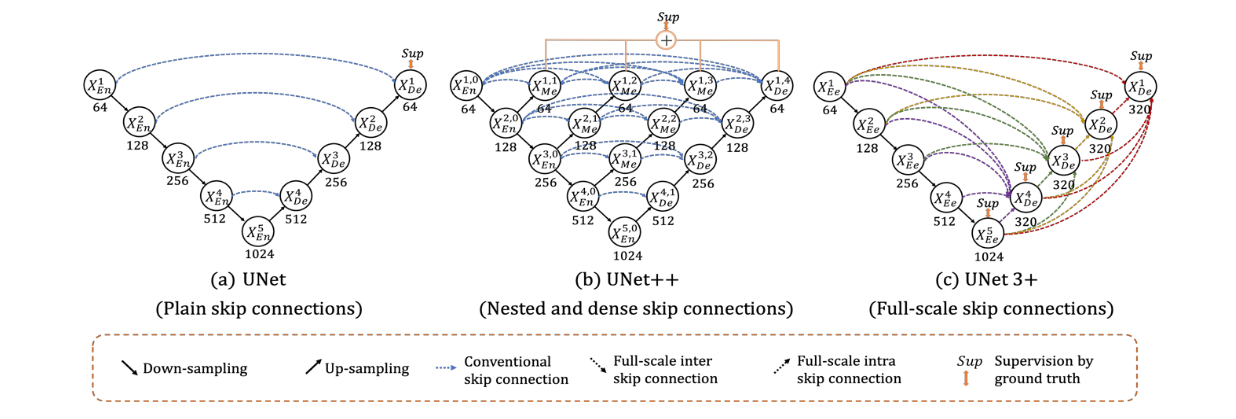
\includegraphics[scale=1.1]{images/unet3p.png}
  \end{center}
  \caption{UNet3+}\label{fig:}
\end{figure}

\section{LinkNet}
\begin{figure}
  \begin{center}
    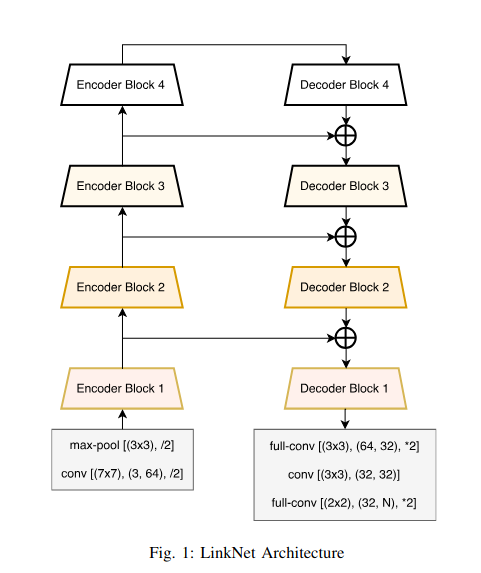
\includegraphics[scale=1.1]{images/linknet.png}
    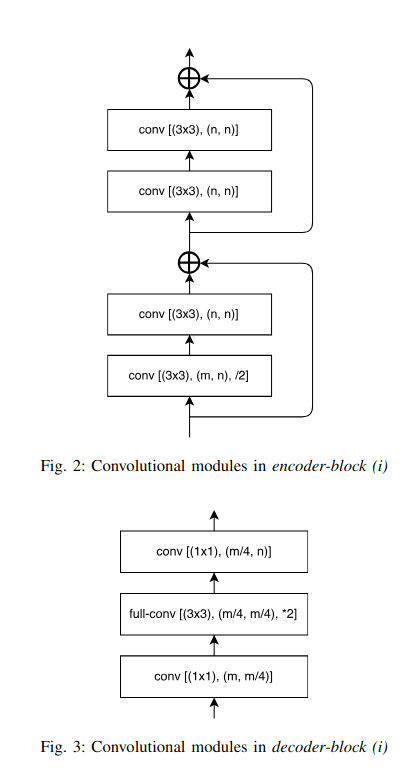
\includegraphics[scale=1.1]{images/linknet-blocks.png}
  \end{center}
  \caption{LinkNet}\label{fig:}
\end{figure}

\section{FPNet}
\begin{figure}
  \begin{center}
    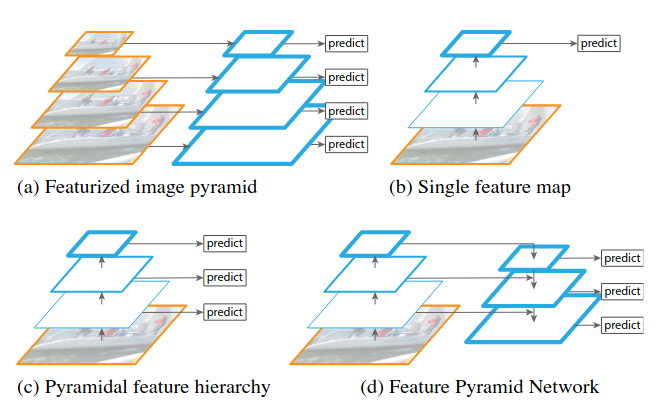
\includegraphics[scale=1.1]{images/fpnet.png}
  \end{center}
  \caption{Feature Pyramid Networks}\label{fig:}
\end{figure}


\section{PSPNet}
\begin{figure}
  \begin{center}
    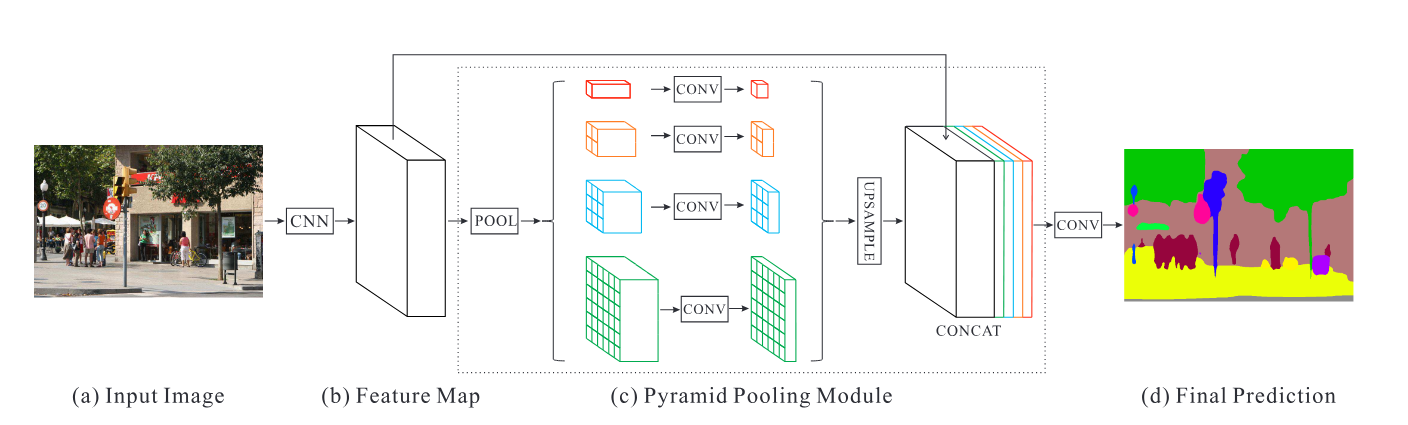
\includegraphics[scale=1.1]{images/pspnet.png}
  \end{center}
  \caption{Pyramid Scene Parser}\label{fig:}
\end{figure}

\section{DeepLabV3+}
\begin{figure}
  \begin{center}
  \end{center}
  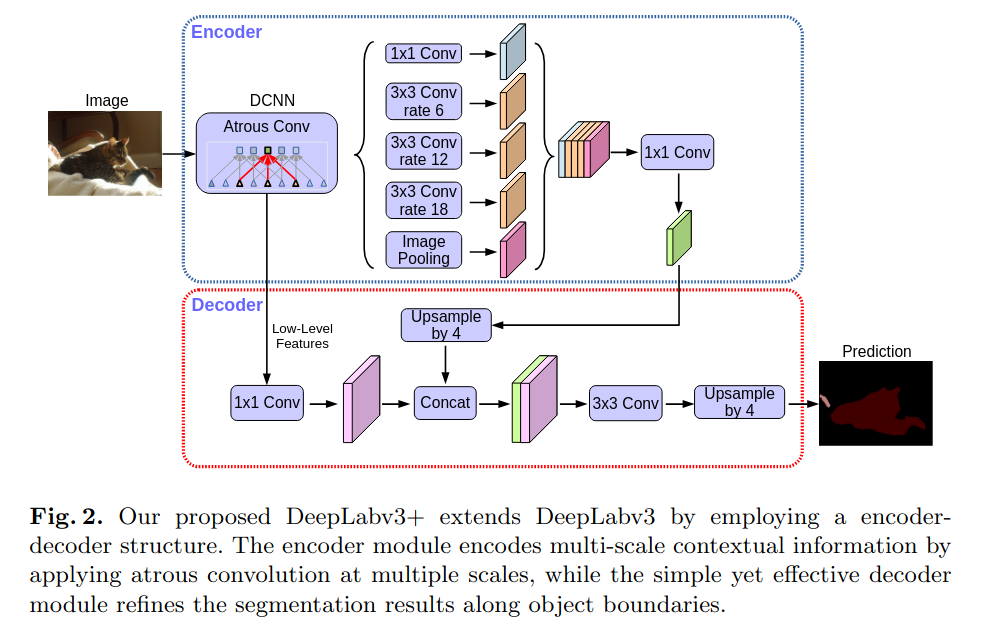
\includegraphics[scale=1.1]{images/deeplabv3p.png}
  \caption{DeepLabV3+}\label{fig:}
\end{figure}

\section{MA-Net}
\begin{figure}
  \begin{center}
    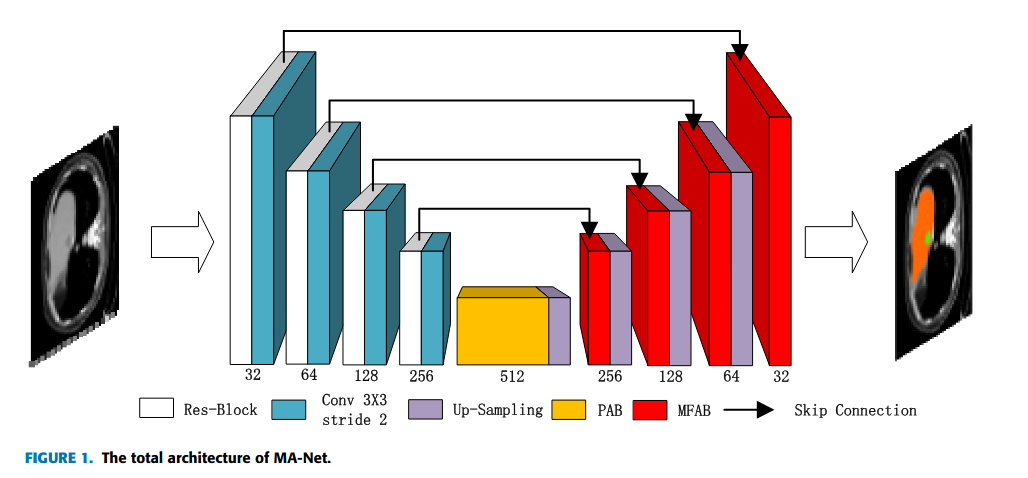
\includegraphics[scale=1.1]{images/manet.png}
  \end{center}
  \caption{Multiscale Attention Network}\label{fig:}
\end{figure}
\begin{figure}
  \begin{center}
    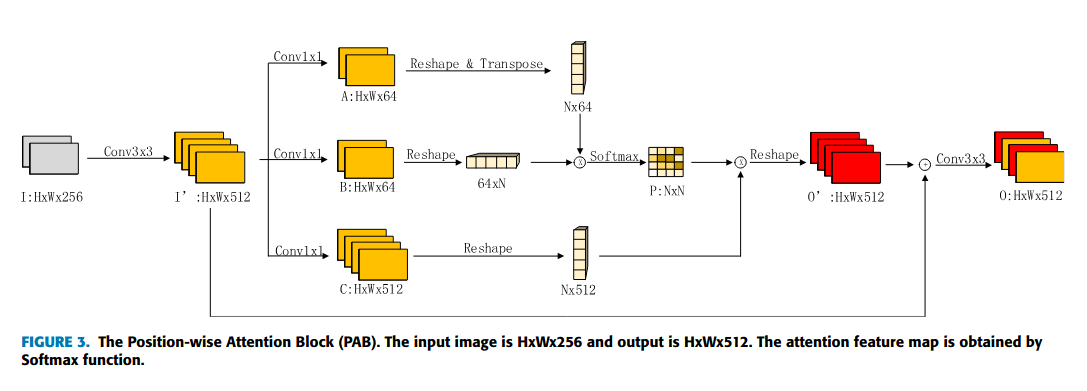
\includegraphics[scale=1.1]{images/pab.png}
  \end{center}
  \caption{Position-wise Attention Block}\label{fig:}
\end{figure}
\begin{figure}
  \begin{center}
    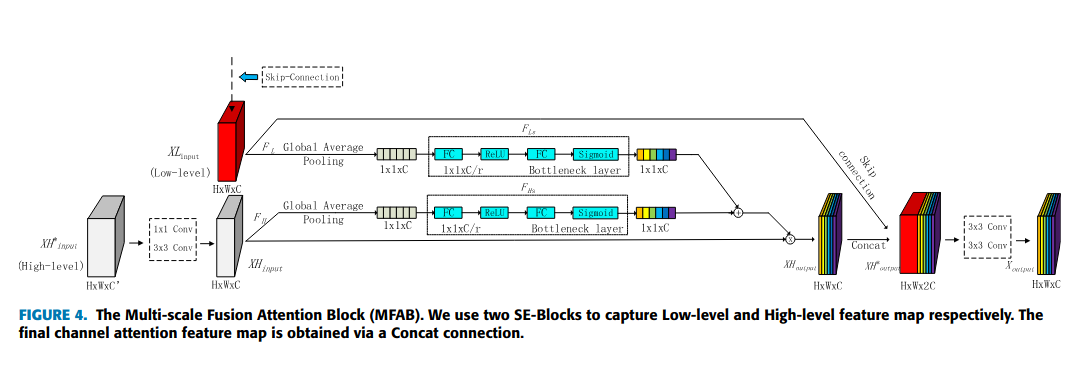
\includegraphics[scale=1.1]{images/mfab.png}
  \end{center}
  \caption{Multiscale Fusion Attention Block}\label{fig:}
\end{figure}

\end{document}
